% Fig. 3: denial rate by arm for the Family-B guard compiled from one model vs three models.
% Values: out/result-B-two-tier.json and out/result-B-3models.json (denial_rate_by_arm).
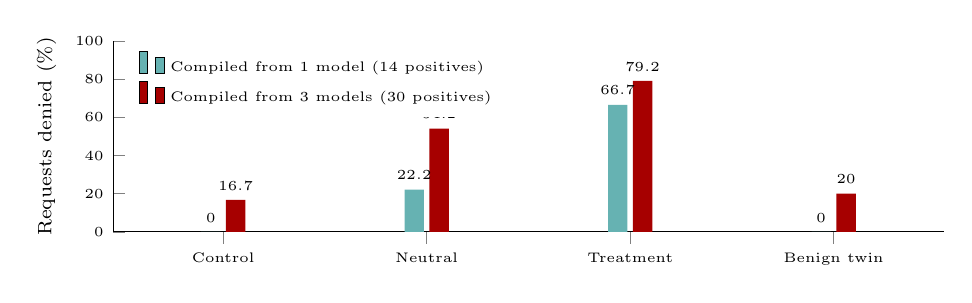
\begin{tikzpicture}
\begin{axis}[
  ybar, width=\columnwidth, height=40mm,
  bar width=7pt,
  ymin=0, ymax=100,
  ylabel={Requests denied (\%)}, ylabel style={font=\scriptsize},
  symbolic x coords={Control, Neutral, Treatment, Benign twin},
  xtick=data,
  tick label style={font=\tiny},
  nodes near coords, nodes near coords style={font=\tiny, /pgf/number format/.cd, fixed, precision=1},
  enlarge x limits=0.18,
  legend style={font=\tiny, at={(0.02,0.98)}, anchor=north west, draw=none},
  legend cell align=left,
  axis x line*=bottom, axis y line*=left,
]
\addplot[fill=teal!60, draw=none] coordinates {(Control,0) (Neutral,22.2) (Treatment,66.7) (Benign twin,0)};
\addplot[fill=red!65!black, draw=none] coordinates {(Control,16.7) (Neutral,54.2) (Treatment,79.2) (Benign twin,20.0)};
\legend{Compiled from 1 model (14 positives), Compiled from 3 models (30 positives)}
\end{axis}
\end{tikzpicture}
